\begin{figure}[t]
\centering
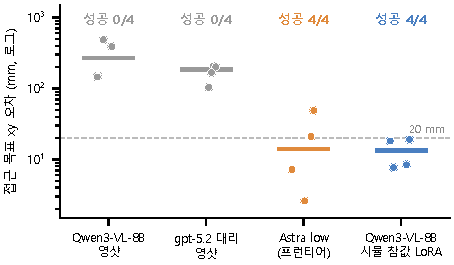
\includegraphics[width=\linewidth]{figures/evidence.pdf}
\caption{\textbf{상위 자리의 위치 읽기 (초기값).} 같은 동기 단독 인터페이스(\texttt{astra-solo@v2})로 머그-트레이 DEV 4편(시드 0·1 $\times$ standard·DR)을 돌렸을 때, 편마다 명령한 접근 목표의 xy 오차 중앙(점)과 네 편의 중앙(막대). 위의 숫자는 폐루프 성공이다. Astra는 파일럿 4편의 값이다(전체 팔 첫 3편도 성공해 합 7/7). 미세조정 8B는 시뮬 참값 라벨로 LoRA 학습한 판이다. 영샷 두 모델은 대상 위치를 10--50\,cm 틀리게 읽었고, 미세조정 8B는 Astra와 같은 범위로 들어왔다. 대리 모델(gpt-5.2)의 값은 오픈 모델 자체의 값이 아니다. 편 수가 4라 방향만 본다. 모든 값은 \tentative{초기값}이다.}
\label{fig:evidence}
\end{figure}
